\chapter{Exemplos}

\section{Exemplo de figura/gráfico}

Na \autoref{fig:exemplo-fig} se encontra um exemplo de imagem inserida no corpo do texto.

\begin{figure} [hbt]
\center
\caption{Exemplo de imagem}
\label{fig:exemplo-fig}
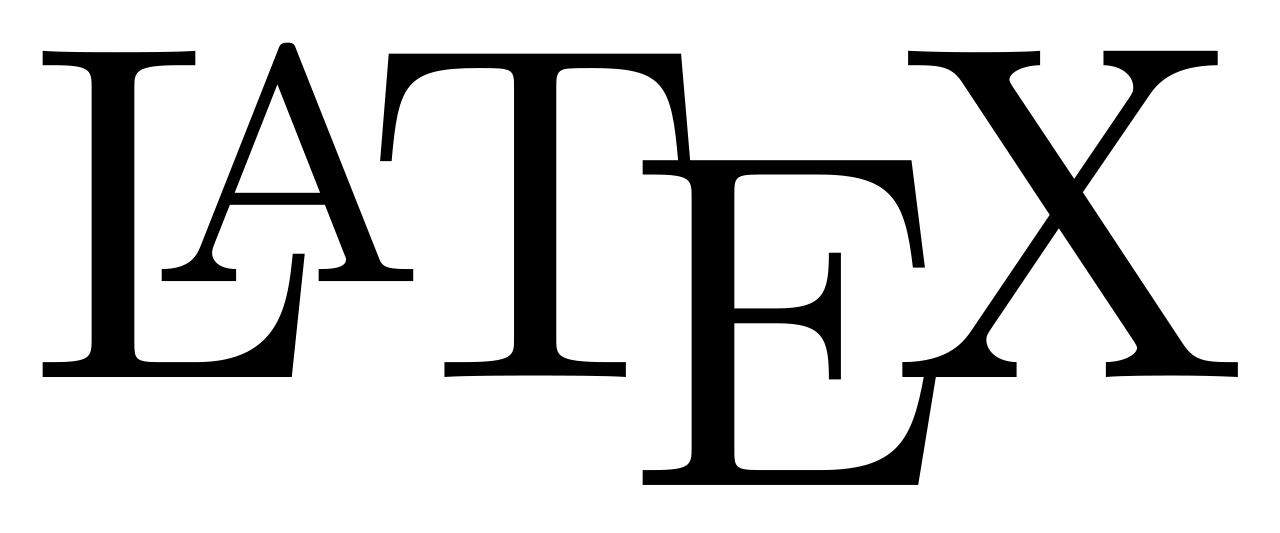
\includegraphics[width=0.6\textwidth]{imagens/LaTeX_logo.png}
\fnote{\citeonline{siteLatex}}
\end{figure}

\section{Exemplo de Tabela}

Na \autoref{tab:exemplo} se encontra um exemplo de tabela inserida no corpo do texto.

\begin{table}[hbt]
\centering
\caption{Primeira tabela de exemplo}
\label{tab:exemplo}
\begin{tabular}{lcccccc}
\hline
\multicolumn{1}{l|}{\textbf{Etapas}}   & \multicolumn{3}{c|}{\textbf{One-DR-F1}}                                                                         & \multicolumn{3}{c}{\textbf{One-DR-F2}}                                                                         \\ \hline
\multicolumn{1}{l|}{\textbf{Sistemas}} & \multicolumn{1}{c|}{\textbf{ViDE}} & \multicolumn{1}{c|}{\textbf{AutoRM}} & \multicolumn{1}{c|}{\textbf{DEPTA}} & \multicolumn{1}{c|}{\textbf{ViDE}} & \multicolumn{1}{c|}{\textbf{AutoRM}} & \multicolumn{1}{c}{\textbf{DEPTA}} \\ \hline
\textbf{Precisão}& 100\%   & 100\%   & 100\%   & 99,2\%   & 99,8\%   & 98,9\%   \\
\textit{\textbf{Revocação}}& 100\%   & 100\%   & 100\%   & 98,3\%   & 99,6\%   &99,6\%   \\ \hline
\end{tabular}
\fnote{\citeonline{prodanov}}
\end{table}

\begin{table}[hbt]
\centering
\caption{Segunda tabela de exemplo}
\label{tab:author-one-dr}
\begin{tabular}{lcccccc}
\hline
\multicolumn{1}{l|}{\textbf{Etapas}}   & \multicolumn{3}{c|}{\textbf{One-DR-F1}}                                                                         & \multicolumn{3}{c}{\textbf{One-DR-F2}}                                                    \\ \hline
\multicolumn{1}{l|}{\textbf{Sistemas}} & \multicolumn{1}{c|}{\textbf{ViDE}} & \multicolumn{1}{c|}{\textbf{AutoRM}} & \multicolumn{1}{c|}{\textbf{DEPTA}} & \multicolumn{1}{c|}{\textbf{ViDE}} & \multicolumn{1}{c|}{\textbf{AutoRM}} & \textbf{DEPTA} \\ \hline
\textbf{Precisão}& 88,6\%   & 95,4\%   & 82,8\%   & 97,8\%   & 99,6\%   & 96,9\%   \\
\textit{\textbf{Revocação}}& 85,4\%   & 96,9\%   & 73,3\%   & 91,5\%   & 98,5\%   & 89,9\%   \\ \hline
\end{tabular}
\fnote{\citeonline{prodanov}}
\end{table}